\chapter{Introduction\label{cha:chapter1}}

This chapter should have about 4-8 pages and at least one image, describing your topic and your concept. Usually the introduction chapter is separated into subsections like 'motivation', 'objective', 'scope' and 'outline'.

\section{Motivation\label{sec:moti}}

Start describing the situation as it is today or as it has been during the last years. 'Over the last few years there has been a tendency... In recent years...'. The introduction should make people aware of the problem that you are trying to solve with your concept, respectively implementation. Don't start with 'In my thesis I will implement X'.

\section{Objective\label{sec:objective}}

What kind of problem do you adress? Which issues do you try to solve? What solution do you propose? What is your goal?
'This thesis describes an approach to combining X and Y... The aim of this work is to...'

\section{Scope\label{sec:scope}}

Here you should describe what you will do and also what you will not do. Explain a little more specific than in the objective section. 'I will implement X on the platforms Y and Z based on technology A and B.'

Conclude this subsection with an image describing 'the big picture'. How does your solution fit into a larger environment? You may also add another image with the overall structure of your component.

'Figure \ref{fig:intro} shows Component X as part of ...' 
\\
\begin{figure}[htb]
  \centering
  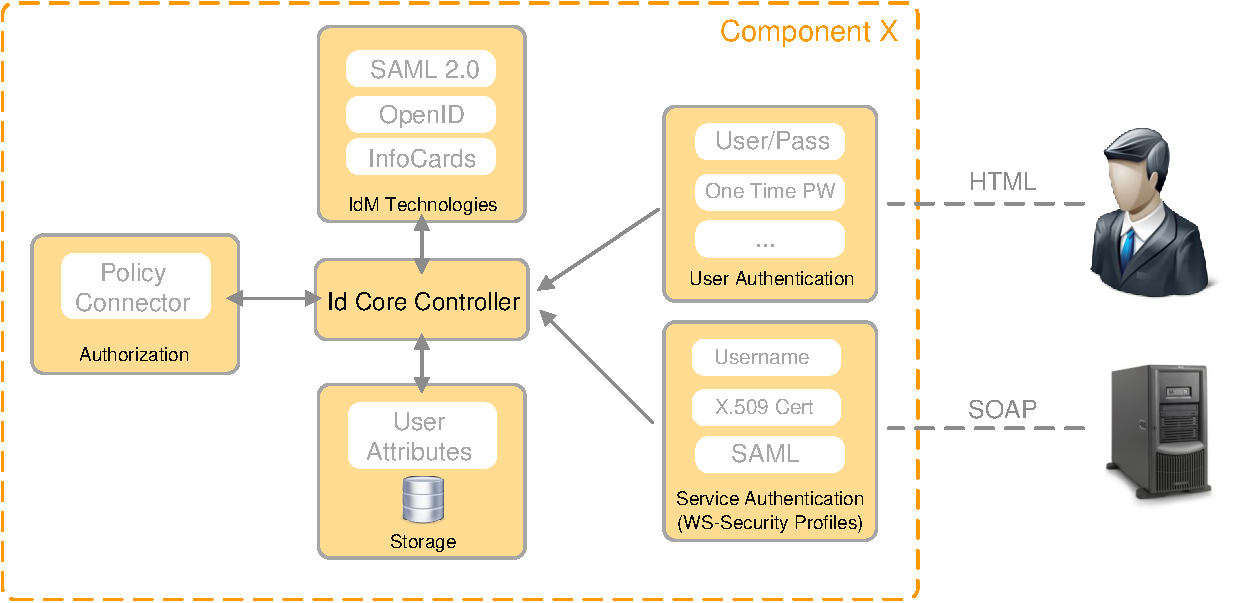
\includegraphics[width=9cm]{intro_example.pdf}\\
  \caption{Component X}\label{fig:intro}
\end{figure}

\section{Outline\label{sec:outline}}

The 'structure' or 'outline' section gives a brief introduction into the main chapters of your work. Write 2-5 lines about each chapter. Usually diploma thesis are separated into 6-8 main chapters. 
\\
\\
\noindent This example thesis is separated into 7 chapters.
\\
\\
\textbf{Chapter \ref{cha:chapter2}} is usually termed 'Related Work', 'State of the Art' or 'Fundamentals'. Here you will describe relevant technologies and standards related to your topic. What did other scientists propose regarding your topic? This chapter makes about 20-30 percent of the complete thesis.
\\
\\
\textbf{Chapter \ref{cha:chapter3}} analyzes the requirements for your component. This chapter will have 5-10 pages.
\\
\\
\textbf{Chapter \ref{cha:chapter4}} is usually termed 'Concept', 'Design' or 'Model'. Here you describe your approach, give a high-level description to the architectural structure and to the single components that your solution consists of. Use structured images and UML diagrams for explanation. This chapter will have a volume of 20-30 percent of your thesis.
\\
\\
\textbf{Chapter \ref{cha:chapter5}} describes the implementation part of your work. Don't explain every code detail but emphasize important aspects of your implementation. This chapter will have a volume of 15-20 percent of your thesis.
\\
\\
\textbf{Chapter \ref{cha:chapter6}} is usually termed 'Evaluation' or 'Validation'. How did you test it? In which environment? How does it scale? Measurements, tests, screenshots. This chapter will have a volume of 10-15 percent of your thesis.
\\
\\
\textbf{Chapter \ref{cha:chapter7}} summarizes the thesis, describes the problems that occurred and gives an outlook about future work. Should have about 4-6 pages.